\section{Software}
\subsection{Architecture}
Along with a new mechanical design, this year saw a complete rebase of existing software. This new software base has had a significant focus on software design principles to ensure the code will be usable both now and in the future. The backbone of the new codebase is a message passing system accomplished through an event/listener design paradigm. Classes are set up to modularize the different stages of data processing, with the creation of each output then activating a callback method within the next step. This pattern provides a greater level of abstration between logical units of the robot. Such a design simplifies the addition and removal of functionality, making it easy to prototype and test new concepts and algorithms. Additionally, because stringent interfaces are a requirement of this framework, simulators can easily be interchanged for functioning components, allowing units to be tested independently.

This redesign also provided an opportunity to reimagine the basic strategy employed for interacting with the world. The new software design has moved away from a purely reactionary system and to a mapping system which includes and synthesizes its current and past knowledge of the world around it to intelligently navigate.

\subsection{Algorithms}
\subsubsection{Vision}
Current software makes increasing use of computer vision over previous years. This increase was largely made possible through the addition of our new stereo camera. This addition has give us a means to translate image information from the camera's frame of reference to real world locations. In addition to allowing the robot to more robustly determine the locations of potential obstacles and barriers, this improvement has also provided an opportunity to gain additional information about the robot's position through the use of visual odometry and other techniques. Many of these added technologies are accomplished through use of the OpenCV framework.
%\vspace*{\baselineskip}

%\textbf{Lane Detection}
\subsubsection*{Lane Detection}
Lane detection is the most fundamental vision task in this competition, While many of the other obstacles may be easily sensed through the use of LIDAR, the nature and position of the white lines make it necessary to use vision to detect them. Our current lane detection algorithm makes use of a number of sequential techniques in order to converge on the location of the lines. The algorithm begins by masking over patterns that match known obstacles with white sections. The image is then segmented and filtered, leaving only pixels that fall within the expected color range of white lines in reasonable lighting conditions. At this point, information about the height above ground and angle of the camera is used to map the remaining points to real-world coordinates for mapping.
%\vspace*{\baselineskip}

%\textbf{Visual Odometry}
\subsubsection*{Visual Odometry}
The visual odometry system employs two separate techniques which complement each other in ability. Visual odometry inherently requires deriving a linkage between the appearance of a point or object in the image and how it relates to its position relative to the robot. The first of the two methods employed accomplishes this through the use of the depth map generated by the stereo camera. By tracking a number of points between frames, using the Harris corners algorithm to identify potential candidates, and seeing how their depth measurements changes, it is possible to determine the change in each of the degrees of freedom between frames. Potential problems caused by inaccuracies in the stereo algorithm or other factors are minimized with multiple random selections of track points for these calculations. 

While this process provides a robust solution, the price of the stereo matching algorithm makes this method computationally expensive, limiting the potential real-time ability of such a technique. The second algorithm used circumvents this issue by assuming that the terrain in front of the robot will not impact that the rotational degrees of freedom of the robot. This assumption trivializes finding the physical correspondences necessary for identifying the change in the other degrees of freedom between frames. This is accomplished by creating a filter to differentiate grassy sections of the image from obstacles and other objects. Once everything else is filtered out, potential interest scores are found for the remainder of the map, and those locations found to be accurate enough are used to determine the change in the non-constrained degrees of freedom. Because the same points are monitored in both images, the relative position of the points to each other should remain constant between frames. By using the calculated update function for robot position between frames, a prediction of where points should appear in the second image may be made. Then by comparing this prediction to the actual end locations, the legitimacy of the assumption can be determined.

\begin{figure}[H]
\begin{minipage}[b]{0.5\linewidth}
\centering
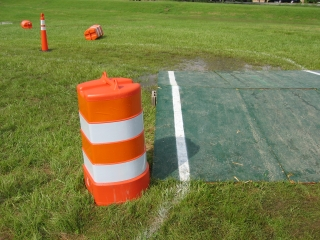
\includegraphics[width=3in]{./Pics/BenCode_534_small.jpg}
\caption{Full Track}
\label{FIG:Track}
\end{minipage}
\hspace{0.1in}
\begin{minipage}[b]{0.5\linewidth}
\centering
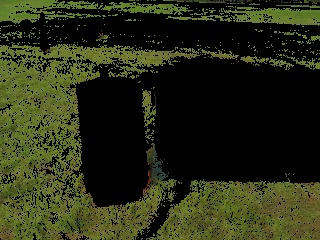
\includegraphics[width=3in]{./Pics/BenCode_534_small_green.jpg}
\caption{Filtered}
\label{FIG:Filtered}
\end{minipage}
\end{figure}

\subsubsection{Mapping}
Mapping is accomplished through the use of the PointCloud library, which allows for efficient creation, storage, and query of 3-D points. This representation integrates information from both the camera and LIDAR into a single representation of the world which can then be used as an input for the path planning algorithm.
\subsubsection{Path Planning}
This year's robot will employ the A* algorithm to perform path planning. This algorithm will use the PointCloud map as an input and will output an optimal path, which will then be translated into an implementable set of movements for the robot to perform.
\subsubsection{Controls}
Two levels of controls algorithms will be used to provide a convenient interface for controlling the motion of the robot. The first of these two algorithms is a closed loop PID controller which will be implemented on the arduino. This algorithm uses the encoder readings that it processes to provide a measure of distance travelled. While this loop provides a fast feedback mechanism, it fails to account for real-world conditions such as wheel slippage and rough terrain. Commands for motion will be dictated by the mapping algorithm as commands to move or turn certain amounts, and the errors accumulating from such causes would undermine the usability of the system. To account for this, an additional control system will be running on the main laptop to ensure that these commands are properly processed. This system will use more accurate measure of the robot position to ensure that these commands have been properly processed, issuing corrective commands to account for the deviations from the required condition until the robot arrives at the proper location.
\subsubsection{Sensor Integration}
The sensors and related algorithms added this year have added an additional level of complexity that did not have to be considered in previous years: how to integrate multiple differing readings of a value. This problem surfaced most noticeably in the area of robot pose tracking, where there are at least four sources of pose information. To accommodate this, a common timing interface was created and integrated throughout the codebase in order to ensure an accurate synchrony among the different pieces of information. All new readings are then passed to a central object responsible for fusing this information into a single estimate of robot pose. This class takes in a number of different data types and converts them all into a common update format. Kalmann filtering is then used to combine all of these readings. The result is a more robust and accurate description of robot pose than could be acquired through the individual use of any of the sensors or techniques.